\documentclass{article}

\usepackage[fleqn]{amsmath} % This package with the fleqn option aligns equations to the left
\setlength{\mathindent}{0pt} % Set indentation from the left margin

\usepackage{amssymb} % Required for math symbols
\usepackage{graphicx} % Required for inserting images
\usepackage{geometry}

\usepackage[section]{placeins}

\usepackage[backend=biber, style=authoryear, citestyle=authoryear]{biblatex}
\addbibresource{references.bib}

\geometry{a4paper, margin=1in}

{
\title{
    
\includegraphics[width=0.34\textwidth]{/Users/mlnick/documents/images/tsukuba-logo.png} \\
    \vspace{2mm}
    \textbf{Numerical Simulation} \\
    \vspace{3mm}    
    Hometask 4
}

\author{Mamanchuk Mykola, SID.202420671}
\date{\today}

}

\usepackage{listings}
\usepackage{color}

\definecolor{codegreen}{rgb}{0,0.6,0}
\definecolor{codegray}{rgb}{0.5,0.5,0.5}
\definecolor{codepurple}{rgb}{0.58,0,0.82}
\definecolor{backcolour}{rgb}{0.99,0.99,0.99}

\lstdefinestyle{mystyle}{
    backgroundcolor=\color{backcolour},   
    commentstyle=\color{codegreen},
    keywordstyle=\color{magenta},
    numberstyle=\tiny\color{codegray},
    stringstyle=\color{codepurple},
    basicstyle=\ttfamily\footnotesize,
    breakatwhitespace=false,         
    breaklines=true,                 
    captionpos=b,                    
    keepspaces=true,                 
    numbers=left,                    
    numbersep=5pt,                  
    showspaces=false,                
    showstringspaces=false,
    showtabs=false,                  
    tabsize=2
}
\lstset{style=mystyle}

\begin{document}

\maketitle


\setlength{\fboxsep}{0pt} % Removes padding around the image
\setlength{\fboxrule}{0.5pt} % Sets the thickness of the border

\section{Derivation of Phase Speed for the Hyperbolic Wave Equation}
We consider the standard wave equation for a uniform medium where the wave speed \( v \) is constant:
\[
\frac{\partial^2 u}{\partial t^2} = v^2 \frac{\partial^2 u}{\partial x^2}
\]
Given the solution form \( u(x,t) = \exp(i(\omega t - kx)) \), we substitute this into the wave equation to analyze the behavior of the wave and derive the phase speed.

\subsection{Substitution and Derivation}
Substituting \( u(x,t) = \exp(i(\omega t - kx)) \) into the wave equation, the derivatives are:
\[
\frac{\partial^2 u}{\partial t^2} = -\omega^2 u, \quad \frac{\partial^2 u}{\partial x^2} = -k^2 u
\]
Plugging these into the wave equation gives:
\[
-\omega^2 u = v^2 (-k^2 u)
\]
Simplifying, we find:
\[
\omega^2 = v^2 k^2
\]
This implies:
\[
\omega = \pm vk
\]

\subsection{Phase Speed Calculation}
The phase speed \( c_p \) of the wave is defined as the speed at which the phase of the wave propagates in space, which is given by the relationship:
\[
c_p = \frac{\omega}{k}
\]
From our earlier result, \( \omega = \pm vk \), substituting we get:
\[
c_p = \frac{\pm vk}{k} = \pm v
\]
Thus, the phase speed of the wave is \( \pm v \), indicating that the wave can propagate both forwards and backwards along the x-axis with speed \( v \).

\subsection{Conclusion}
The derivation confirms that the phase speed of the wave described by the hyperbolic wave equation \( u(x,t) = \exp(i(\omega t - kx)) \) is equal to the constant wave speed \( v \) in the medium. This result is consistent with the physical expectation for waves in a homogeneous isotropic medium.

\section{Derivation of the Dispersion Relation for the Hyperbolic Equation}
We analyze the dispersion relation of the hyperbolic equation using a numerical approximation prescribed by the staggered leapfrog scheme. The numerical scheme approximates the second-order hyperbolic wave equation as follows:
\[
u_j^{n+1} - 2u_j^n + u_j^{n-1} = \frac{v^2 \Delta t^2}{\Delta x^2} \left(u_{j+1}^n - 2u_j^n + u_{j-1}^n\right)
\]

\subsection{Analytical Approach}
Given \( u(x,t) = \exp(i(\omega n\Delta t - k j\Delta x)) \), we substitute this ansatz into the finite difference equation. By expressing all terms in the form of the exponential ansatz and simplifying, we derive the following expression:
\[
\exp(i\omega\Delta t) - 2 + \exp(-i\omega\Delta t) = \frac{v^2 \Delta t^2}{\Delta x^2} \left(\exp(ik\Delta x) - 2 + \exp(-ik\Delta x)\right)
\]
Using Euler's formula where \( \exp(ix) + \exp(-ix) = 2\cos(x) \), we rewrite the equation as:
\[
-2 + 2\cos(\omega\Delta t) = \frac{v^2 \Delta t^2}{\Delta x^2} \left(-2 + 2\cos(k\Delta x)\right)
\]
This simplifies to:
\[
\cos(\omega\Delta t) = 1 - \frac{v^2 \Delta t^2}{\Delta x^2} \left(1 - \cos(k\Delta x)\right)
\]
Using the identity \( \sin^2(x) = \frac{1 - \cos(2x)}{2} \), we obtain:
\[
\cos(\omega\Delta t) = 1 - 2 \frac{v^2 \Delta t^2}{\Delta x^2} \sin^2\left(\frac{k\Delta x}{2}\right)
\]

\subsection{Dispersion Relation}
By solving for \( \omega \), considering \( \cos(\omega\Delta t) = \cos(\theta) \) implies \( \omega\Delta t = \pm \theta \), we derive:
\[
\omega\Delta t = \pm 2\sin^{-1}\left(\frac{v\Delta t}{\Delta x} \sin\left(\frac{k\Delta x}{2}\right)\right)
\]
Thus, the dispersion relation in terms of \( \omega \) as a function of \( k \) is:
\[
\omega = \pm \frac{2}{\Delta t}\sin^{-1}\left(\frac{v\Delta t}{\Delta x} \sin\left(\frac{k\Delta x}{2}\right)\right)
\]

\subsection{Conclusion}
This dispersion relation indicates how the angular frequency \( \omega \) varies with the wave number \( k \) in the numerical scheme. It highlights the dependence of the wave speed on the grid spacing \( \Delta x \) and the time step \( \Delta t \), which are crucial for accurately capturing the wave dynamics in a discrete computational domain.

\section{Comparison of Dispersion Relations}

\subsection{Objective}
The objective was to compare the dispersion relations derived from both analytical and numerical methods, specifically for the staggered leapfrog scheme, and analyze the discrepancies introduced by numerical discretization.

\subsection{Methodology}
The dispersion relations were evaluated for waves modeled by the hyperbolic wave equation, using both analytical solutions and numerical approximations obtained through the staggered leapfrog scheme. The wave number spectrum was analyzed up to the Nyquist limit, focusing on how different ratios of \( \frac{v\Delta t}{\Delta x} \) influence the dispersion characteristics.

\subsubsection{Analytical Relation}
The analytical dispersion relation is given by:
\[
\omega = v k
\]
where \( \omega \) is the angular frequency, \( v \) is the wave speed, and \( k \) is the wave number.

\subsubsection{Numerical Relation}
The numerical relation was derived from the finite difference approximation:
\[
\omega \Delta t = 2 \sin^{-1}\left(\frac{v\Delta t}{\Delta x} \sin\left(\frac{k\Delta x}{2}\right)\right)
\]
This was evaluated for \( \frac{v\Delta t}{\Delta x} \) ratios of 0.5, 0.25, and 0.1.

\subsection{Results}
The comparison was visualized in a plot showing both the analytical and numerical dispersion relations, highlighting the deviations of the numerical model from the true physical behavior as the wave number approaches the Nyquist limit. This is attributed to the finite difference discretization, particularly impacting the accurate representation of wave propagation at higher wave numbers.

\vspace{3mm}
The plot is provided on the next page.

\newpage

\begin{figure}[!]
    \centering
    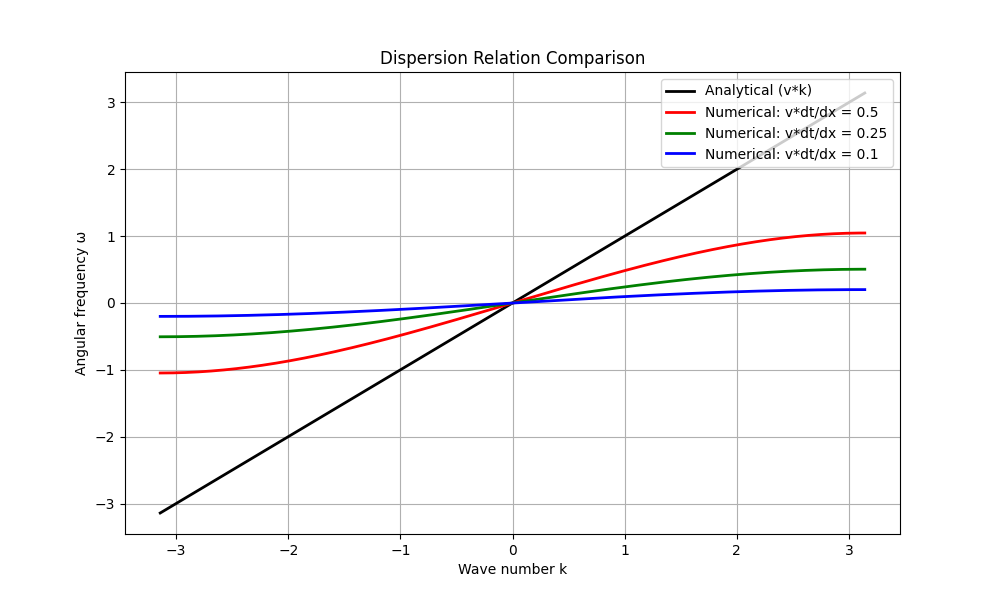
\includegraphics[width=1\textwidth]{materials/Figure_1.png}
    \caption{Dispersion relations comparing analytical (black line) and numerical schemes with different \( \frac{v\Delta t}{\Delta x} \) values.}
    \label{fig:dispersion_relations}
\end{figure}

\subsection{Conclusion}
The analysis demonstrated significant differences between the analytical and numerical dispersion relations, especially near the Nyquist wave number. These discrepancies are crucial for understanding the limitations and necessary adjustments in numerical simulations to enhance model accuracy, particularly in scenarios where high resolution is required.

\subsection{Python Plotting Script}
The Python code used to generate the plots and conduct the analysis is provided below.

\begin{lstlisting}[language=python]
    import numpy as np
    import matplotlib.pyplot as plt
    
    # Parameters
    v = 1  # Wave speed
    dx = 1  # Spatial resolution (Delta x)
    dt = 1  # Time step (Delta t)
    k = np.linspace(-np.pi, np.pi, 500)  # Wave number range from -pi to pi
    
    # Analytical Dispersion Relation
    omega_analytical = v * k
    
    # Numerical Dispersion Relations for different v*dt/dx ratios
    ratios = [0.5, 0.25, 0.1]
    colors = ['r', 'g', 'b']  # Colors for different plots
    
    # Plotting
    plt.figure(figsize=(10, 6))
    plt.plot(k, omega_analytical, 'k-', label='Analytical (v*k)', linewidth=2)
    
    # Calculate and plot numerical dispersion relation for each ratio
    for ratio, color in zip(ratios, colors):
        omega_numerical = 2 * np.arcsin(ratio * np.sin(k / 2)) / dt
        plt.plot(k, omega_numerical, color, label=f'Numerical: v*dt/dx = {ratio}', linewidth=2)
    
    # Formatting the plot
    plt.xlabel('Wave number k')
    plt.ylabel('Angular frequency w')
    plt.title('Dispersion Relation Comparison')
    plt.legend(loc='upper right')
    plt.grid(True)
    plt.show()        
\end{lstlisting}

\section{Limitations of Numerical Approximations in Wave Propagation}

Numerical approximations of the wave equation, particularly finite difference methods like the staggered leapfrog scheme, are crucial for solving many physical problems computationally. However, there are specific scenarios where these methods fail to deliver accurate results due to inherent limitations:

\subsection{Aliasing and Nyquist Limit}
The finite difference methods can introduce significant errors near the Nyquist limit, where the wave number \(k_{Nyquist} = \pi/\Delta x\). Beyond this limit, the discretization fails to capture the wave correctly, leading to aliasing effects. This phenomenon occurs because the discrete samples cannot represent higher frequencies accurately, resulting in their misinterpretation as lower frequencies.

\subsection{High Wave Number Regions}
At high wave numbers, the numerical scheme's dispersion relation deviates significantly from the physical dispersion relation. This discrepancy arises because the sinusoidal components used in the discretization do not scale linearly with the wave number, causing phase and speed errors in the numerical solution.

\subsection{Sharp Gradients and Discontinuities}
Numerical methods often struggle with problems that exhibit steep gradients or discontinuities, such as shock waves. Traditional finite difference schemes can result in spurious oscillations or numerical instability in these regions, requiring more sophisticated approaches like higher-order methods or adaptive mesh refinement to handle such complexities.

\subsection{Stability and Accuracy}
The stability of numerical methods is governed by the CFL condition, which relates the time step size \(\Delta t\) and the spatial step size \(\Delta x\) to the wave speed \(v\). Inadequate ratios of \(\Delta t/\Delta x\) can lead to inaccurate wave speeds and even numerical instabilities, limiting the method's applicability to certain problems.

These limitations underscore the need for careful selection of numerical methods based on the specific requirements and characteristics of the physical problem at hand. It also highlights the importance of numerical analysis in ensuring the reliability and accuracy of computational simulations.

\section*{References}
\begin{enumerate}
    \item \textbf{Mamanchuk N., University of Tsukuba}, Github, \today. Available online: \url{https://github.com/RIFLE}
    % \item \textbf{Company}, Name of Work, year. Available online: \url{https://...} [Accessed: yyyy-mm-dd]
\end{enumerate}

\end{document}
